\begin{center}
	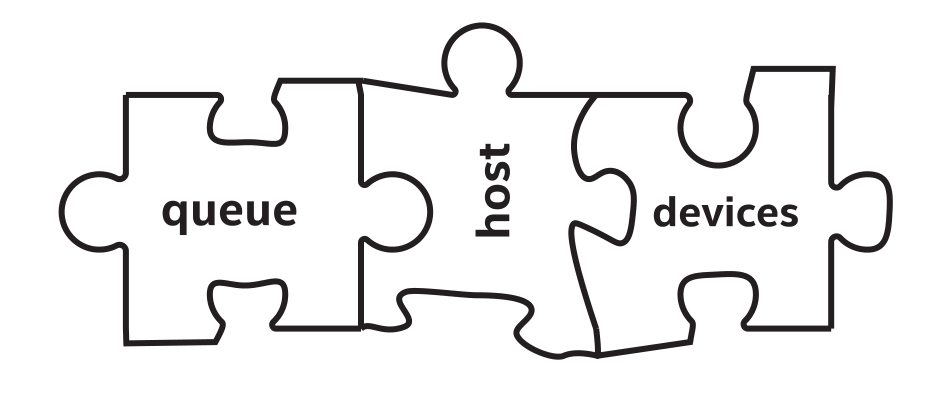
\includegraphics[width=0.5\textwidth]{content/chapter-2/images/1}
\end{center}

并行编程并不是真的在快车道上行驶,而是在所有车道上快速行驶。这一章是关于能够把代码放到可以执行的地方执行,并且选择在合适的时候启用异构系统中的计算资源。因此,需要知道有哪些计算资源(找到它们),并让它们工作(在上面执行代码)。\par

可以控制代码的执行位置——可以控制内核代码运行的设备。SYCL为异构编程提供了框架,代码可以在主机CPU和设备的混合上执行。决定代码在何处执行的机制,对于我们理解和使用异构系统非常重要。\par

本章描述了代码可以在什么地方,什么时候执行,以及用来控制执行位置的机制。第3章将了解如何管理数据,使其在代码执行时使用,然后第4章返回到代码本身,讨论内核代码的编写。\par